\chapter{Motivation}
Model Based Engineering is the cool new thing in the domain of electrical and software engineering. The Unified Modelling Language (UML) offers a large set of Modelling Elements and Diagrams and is also extensible. It can be used to describe almost everything. One can Model verry detailed and describe a System bit by bit and at the same time a simple Diagram can give a quick and intuitive overview over the System. Nevertheless Modelling in UML is an effort that needs to pay off to be economic. UML modelling is not an end unto itself. 
\section{A real world problem at Airbus}
At Airbus Buxtehude Model Based engineering shall soon replace the traditional requirement driven Engineering approach. There are three main benefits that shall be realized with model based engineering. The first one is that the Model can be used for documentation purpose and several documents required by regulatory bodies can be generated from it. The second is the generation of source code itself from the model. And last but not least the model can also serve as a test model from which all necessary test cases for the software can be deduced.\\
For modelling behaviour and control flow of C functions UML Activities shall be used. There exists already a proprietary code generator, which generates a folder structure, C source code files and C header files from UML structural model elements and fills function bodies with code generated from UML Activities. The fact that the code is generated does not make it fault free. We still need to validate the generated code by unit tests. It is not a good idea to generate the source code as well as the unit test from the same model. We need some independence between the implementation and the corresponding unit tests. Writing the complete unit test code by hand is cumbersome. Generating Unit Tests from a complete new model that is build independently from the model used for code generation still imposes some unnecessary work. The Idea is to share the structure of the Activity between code generation and test generation. While the code generation uses procedural C code snippets that are embedded in the model the test generation only relies on embedded declarative OCL constraints. By using two different programming paradigms as input for code generation and test generation we assure some independence between the generated implementation and unit tests.
\section{Idea of this Thesis}
In this thesis we want to focus on generating unit tests from UML Activities with embedded OCL constraints.



 To be precice at airbus the decicion was to use UML Activities for modelling behavior and controll flow of C functions for embedded Systems. Basically we want to harvest the benefits from Model Based Engineering by building tool support to generate a test suite for a C function. The generated Test Suite should of course be complete according to some coverage criteria to be selected by the user. And it needs to integrate with the currently used Modelling tools. There is no use in having a Tool working with models when you can not use the models from your standard modelling environment but have to build new models. Since there is not already some tool available fulfiling oure needs we decided to use Model transformations to transform the UML Model stepwise into a more precice mathematical Model in which we can generate all necessary inputdata via constraint solving, mathematical seach and Optimization. A UML Activity Diagram will be transformed into a Constraint System. This Constraint System can now be solved for any possible path in the Activity resulting in possible input arguments for the C function that will cover the given control flow path. In a last step we are writing the calculated input arguments into a Unit Test code that can be compiled and executed to directly test the given function. 
\subsection{Behavioural Modelling}
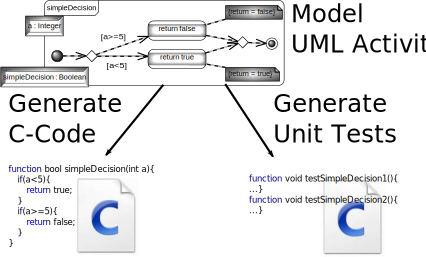
\includegraphics[width=0.5\textwidth]{./pics/Activity2Code+Tests.png}
\subsection{Generating Unit Tests from Behavioural Model}
Explain Model Based engineering at Airbus Buxtehude with Component structure of the software and code generation as well as Test generation from a Model.

Give the short overview over the complete thesis